% !TeX root = ../../../main.tex
\begin{figure}[htbp]
\begin{ChFiveFloatBody}

  \centering
  \begin{minipage}[t]{0.49\linewidth}
    \centering
    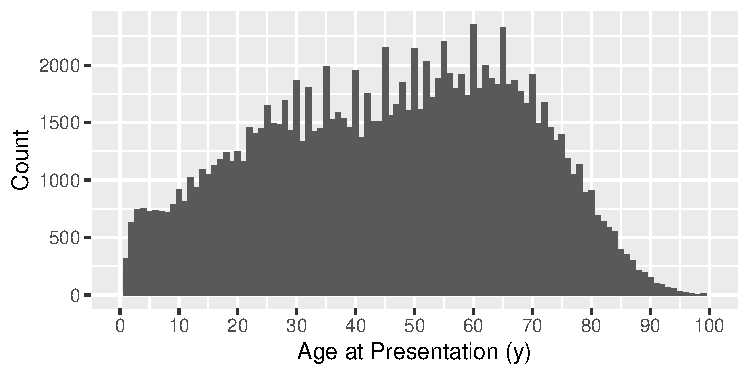
\includegraphics[width=\linewidth]{Chapters/chapter-05/images/Scientific_data/Plots_tables/125k_age.pdf}
  \end{minipage}\hfill
  \begin{minipage}[t]{0.49\linewidth}
    \centering
    \scriptsize
    \begin{tabular}{l r}
      \toprule
      \textbf{Characteristic} & \textbf{Percent (\%)}\\
      \midrule
      \multicolumn{2}{l}{\textbf{Sex}}\\
      \quad Male & 52\\
      \quad Female & 47\\
      \quad Not Specified & 1\\
      \midrule
      \multicolumn{2}{l}{\textbf{Ethnicity}}\\
      \quad White/Caucasian & 5\\
      \quad Asian & 3\\
      \quad African & 1\\
      \quad Other & 2\\
      \quad Not Specified & 89\\
      \bottomrule
    \end{tabular}
  \end{minipage}
  
  
  

\end{ChFiveFloatBody}
\caption{\ChFiveRebuttal{Age distribution and LLM-mapped/extracted demographic descriptors for 124{,}349 PMOA-TTS case reports.}}\ChFiveFloatLabel{ch05:fig:demo}
\end{figure}